\documentclass[12pt, twocolumn]{article}
\usepackage{graphicx}
\usepackage{verbatim}
\setlength{\oddsidemargin}{0in}
\setlength{\evensidemargin}{0in}
\setlength{\textheight}{9in}
\setlength{\textwidth}{6.5in}
\setlength{\topmargin}{-0.05in}


\def \binom{ \atopwithdelims ( )}

\input{macros}

%typeset as follows (can leave off the file's tex/dvi extensions here):
%  latex $filename
%  bibtex $filename
%  latex $filename
%  latex $filename
%  dvipdf $filename  (alternatively MacTex has "dvipdft" executable here)
%...share the $filename.pdf

\parindent 0pt             %No indentation at the start of each paragraph
\parskip 8pt               %5pt is the gap between paragraphs

\begin{document}

\title{Analysis of Compiler Optimizations in Power Consumption}
\author{%  Authors, affiliations, and email addresses go here, like this:
Hari Amoor - Programming Languages \& Compilers II\\
{\ttfamily\normalsize amoor.hari@rutgers.edu}\\
} % end author section
\date{February 21, 2020}


\maketitle

\begin{abstract}

  Energy conservation is an important goal for compilers in various settings, including embedded or otherwise power-constrained systems. \\
  \newline
  In this write-up, we (1) analyze how power and energy consumption is impacted by different optimization levels, and (2) showcase a C program intended to consume as much power as possible for a fixed time period.
  
\end{abstract}

\section{Power Consumption of GCC-optimized Programs}

% Put some text and always cite all your references\cite{vanmeter2006aiq}.
% And some more text text text.

% And a list is list this:
% \begin{itemize}
% \item Foo
% \item Bar
% \item Baz
% \end{itemize}

We present \textit{Fib}, a C program (given as specified on TX cluster) that creates multiple processes with the Unix $\it{fork}$ system call. Each process generates random values for some $n \in \mathbb{N}$ and computes the $n^{\text{th}}$ Fibonacci number with respect to some initial state defined in $\it{main.h}$ with the C $\it{double}$ type (the classical Fibonacci sequence has initial state $f(1) = f(2) = 1$). \\
\newline
Each process also writes the computed value to a specified file. The computation of the "Fibonacci" numbers is done in each process in $\mathcal{O}(n)$ time and space complexity; in particular, the implementation uses tail-recursion and floating-point arithmetic. \\
\newline
Consider the power consumption of \textit{Fib} compiled with GCC under optimization options \textit{-O1}, \textit{-O2}, and \textit{-O3}. Figure 1 indicates that \textit{Fib} consumes at most over 9.8 watts of power under \textit{-O1}, whereas it consumes under 7.1 watts when compiled with \textit{-O2}.
\begin{figure}[t]
  \centering
  
  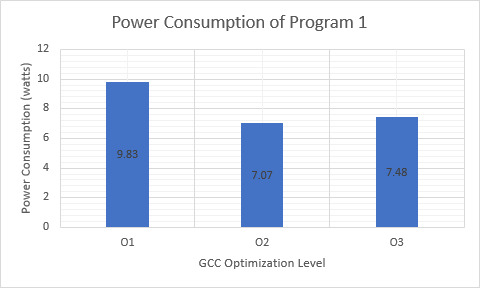
\includegraphics[scale=0.65]{images/fig1.jpg}

  \caption{Comparison of \textit{Fib} under different levels of compiler optimization}
  \label{fig:1}
\end{figure}

The generated assembly code reveals that the program runs recursively as intended when compiled with \textit{-O1}, whereas it runs iteratively when compiled with \textit{-O2}. This suggests that one reason for the decreased power consumption is the tail-recursion optimization conducted by the compiler under \textit{-O2}. Such an explanation stands to reason on the basis that provisioning stack memory for $\mathcal{O}(n)$ recursive calls, as the program does under \textit{-O1}, is very power-intensive relative to the equivalent iterative algorithm. \\
\newline
The increased power consumption with \textit{-O3} relative to \textit{-O2} is less clear. However, GCC enables optimizations like \verb|-ftree-loop-vectorize| involving loop-vectorization that \textit{-O2} does not. Therefore, conjecturally, it is probable that optimizations involving vectorization and unsafe floating-point arithmetic enabled in \textit{-O3} result in greater speed at the tradeoff of slightly greater power consumption.

\section{Maximum Possible Power Consumption}

We showcase \textit{Mandelbrot}, a program designed to consume the maximum possible amount of power. \textit{Mandelbrot} computes an image file containing a Mandelbrot fractal, then removes the file; constants describing how many times \textit{Mandelbrot} does this, and how many processes it does this on, are parametrized with macros in \verb|main.h|. \\
\newline
\textit{Mandelbrot} causes at most a 7.76 watt consumption of energy. It utilizes complex floating-point arithmetic, dynamic memory usage, file I/O, and multiprocessing, each of which result in heavy power-utilization.

\section{Conclusion}
At a high level, optimizing compilers such as GCC optimize for performance not only w.r.t. speed, but also other metrics such as memory and power or energy consumption. \\
\newline
Low-complexity optimizations such as constant propagation and variable elimination can result in strictly-better performance, i.e. improvements in some metrics without any regressions in others, but usage of higher-complexity optimizations such as the ones called for by the \textit{-O3} option can result in tradeoffs between different optimization targets. Case in point, there are many optimizations called for in \textit{-O3} that result in greater speed at the cost of increased power consumption.
\end{document}
